\documentclass[a4paper]{article}
\usepackage{graphicx}
\usepackage{amsmath}
\usepackage{centernot}
\usepackage{listings}

\begin{document}

\title{\textbf{Game Description}}
\author{Nahid Mahbub}
\date{}
\maketitle

\begin{abstract}
The document contains a description of a Game Exercise given by Carma to assess candidate's level of understanding of object design and the Java language.
\end{abstract}

\section*{Game Description}
A playing area is 100m x 100m. A game has a referee and 10 players. A player moves 1m every second and starts out in a random place on the playing area. A referee has to give a yellow card to a player if that player moves within 2m of another player. It is the player that moves to within 2m gets the card. If a player gets 2 yellow cards, the player is ejected from the game for 10 seconds. When a player is off 10 secs the player needs to ask the referee if they are eligible to play again. The referee will let the player return to playing the first time this happens, but not subsequent times. The last player left playing is the winner.

\section*{Assumptions}
Assumptions are following :
\begin{itemize}
\item A playing area is a 2 dimensional grid of 100 x 100 cells.
\item A player have four moves : left, right, up and down
\item Each cell is 1$m^{2}$ block, so each move is 1m.
\item In our parying grid distances are measured as Manhattan distances
\end{itemize}

\section*{Class Diagram}
Figure \ref{fig:permission} visualizes main classes of the application. As shown in the class diagram, GameEmulator has the main method, the entry point of this java console application. From this method emulate method is called and the emulation starts.
\begin{figure}[ht!]
\centering
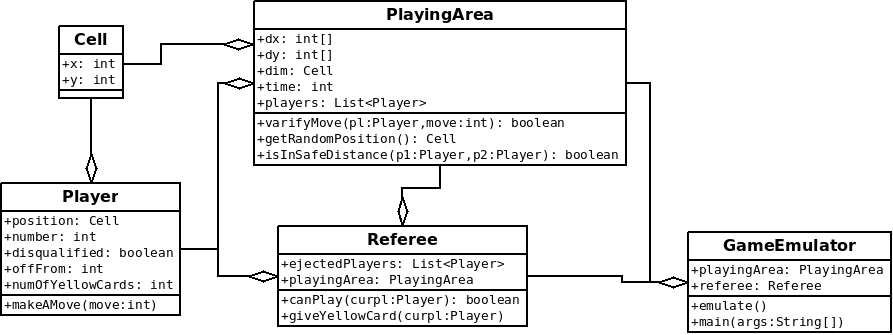
\includegraphics[width=1.2\textwidth]{class_diag.png}
\caption{Class diagram\label{fig:permission}}
\end{figure}

\section*{How the application works}
The application has model objects in $ma.car.exercise.model$ packages, utility class in $ma.car.exercise.util$ and the emulator in $ma.car.exercise.emulator$ packages. The emulator class is responsible foe creating required model objects and making each step of the game. A time counter is there in PlayingArea object which tracks how many seconds spend. In a random setting, it takes more than 60 thousand seconds to obtain a result from this emulator. Listing \ref{CodeSnippet} provides a snippet the of output generated by the application.

\begin{lstlisting}[caption=App output snippet,label=CodeSnippet]
Player 3 is ejected at 48 sec
Player 5 is ejected at 50 sec
Player 10 moved to (6,7)
Playing time : 56
Player 3 is ejected at 48 sec
Player 5 is ejected at 50 sec
Player 10 moved to (5,7)
Playing time : 57
Player 3 is ejected at 48 sec
Player 5 is ejected at 50 sec
Player 10 moved to (4,7)
Playing time : 58
Player 3 removed
Player 5 is ejected at 50 sec
Player 10 moved to (4,6)
Playing time : 59
Player 5 is ejected at 50 sec
Player 10 moved to (4,7)
Playing time : 60
Player 5 removed
Player 10 moved to (4,8)
Playing time : 61
Player 10 win
\end{lstlisting}

\section*{How to build}
Provided Zip archive has source code and an automated build script to build and execute the application. You need to install Apache Ant to build the application. Issue $ant$ command to see available targets (eg. $ant run$ to execute the application).

\section*{Run without Ant}
An executable jar file in $dist/carma.gameexercise.jar$. is also provided in the Zip archive. To run this jar file issue ``java -jar dist/carma.gameexercise.jar'' command form terminal.

\section*{Testing}
Three different tests are provided under $ma.car.exercise.test$ package in $src/java/test/$ folder. One for testing utility methods, one for PlayingArea and last one for testing Referee object. Invoking ``ant unit-test'' will execute this junit based unit testing scripts.

\end{document}

